\section{Count of persons data}
This section discusses the properties of the recorded data as well as its suitability for context prediction.
\subsection{Properties of the data}
\label{sec:PassengerDensityData}

In order to model the passenger density an understanding of the available data is necessary. In this section the data, visible pattern and other features are discussed.

Figure~\ref{fig:rawData_week} illustrates exemplary the available values of a camera and week. The PdG service times are visible due to the low passenger density level between 01:00 and 05:00 on weekdays.

The figure details the passenger density data observed by one particular out of the 20 installed CCTV cameras (indexed with ID 700).
Due to the acquisition process in which density information is extracted from circular snippets 
\marginpar{
\begin{figure}%[htbp]
  \begin{center}
  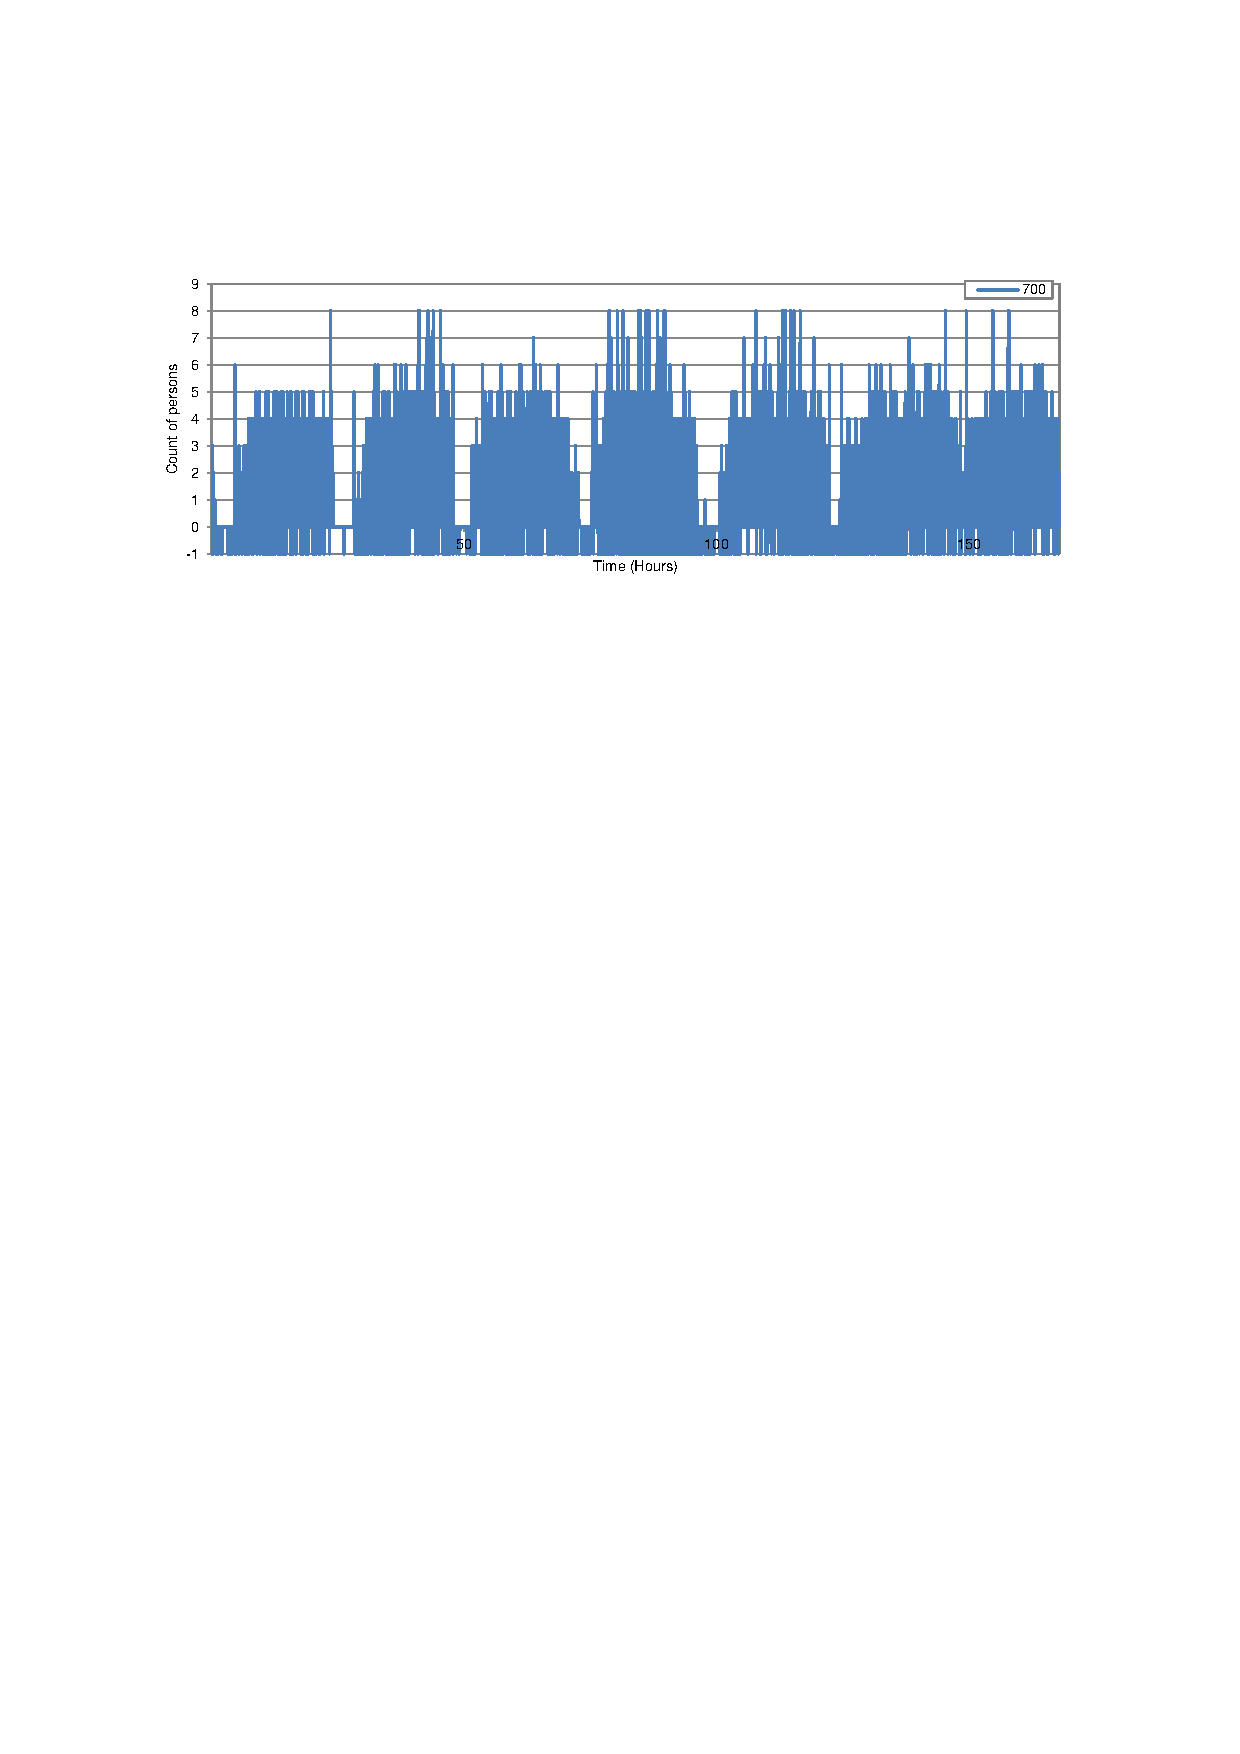
\includegraphics[height=\marginparwidth, angle=270]{Figures/rawData_week.pdf}
  \caption{Passenger density distribution of one camera during one week.}
  \label{fig:rawData_week}
  \end{center}
\end{figure}
}
of the various cameras (see description of the recording process above), for each camera one estimate on passenger density is computed every one minute, leading to a total of 1440 samples per camera and per day.
Again, due to the data processing operation, samples taken are not simultaneous for different cameras but taken sequentially so that pairwise samples are misaligned by at most 30~seconds.

The passenger density is highly correlated for the distinct cameras installed in the metro system which reflects that a specific share of the passengers is always observed by any of the cameras.
This is depicted in Figure~\ref{figureHours}.

The figure displays the mean aggregated passenger density over the course of several days and observed by four different CCTV cameras (with IDs 711, 716, 7004 and 7112).

A single point in this figure reflects the mean aggregated passenger density over a window of 30 minutes with an overlap of 15 minutes.
% \marginpar{
% \begin{figure}
% \begin{center}
%  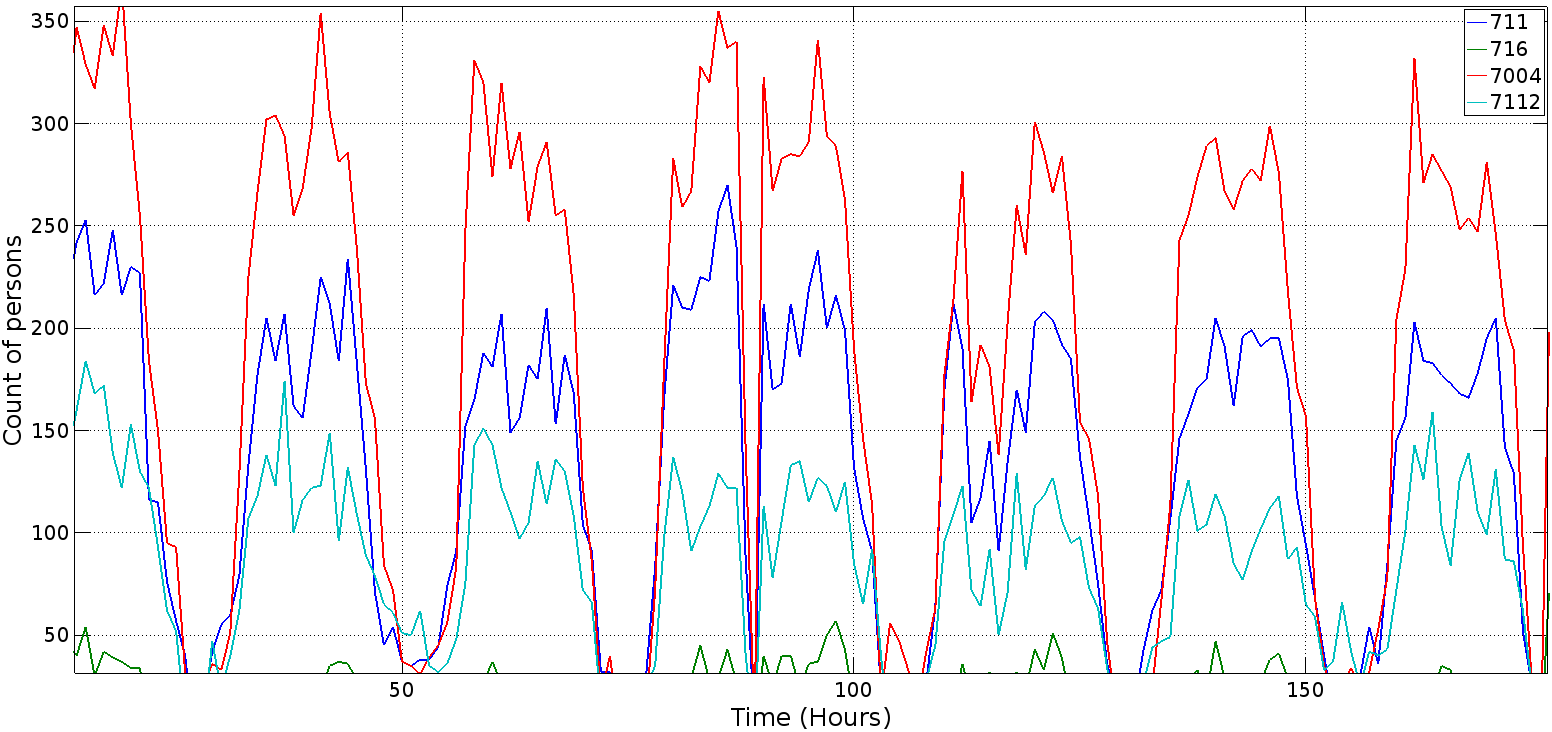
\includegraphics[height=\marginparwidth,angle=270]{Figures/Figure_PersonCount_Hours.png}
%  \caption{todo}
%   \label{figureHours}
%   \end{center}
% \end{figure}
% }
\begin{figure}
\begin{center}
 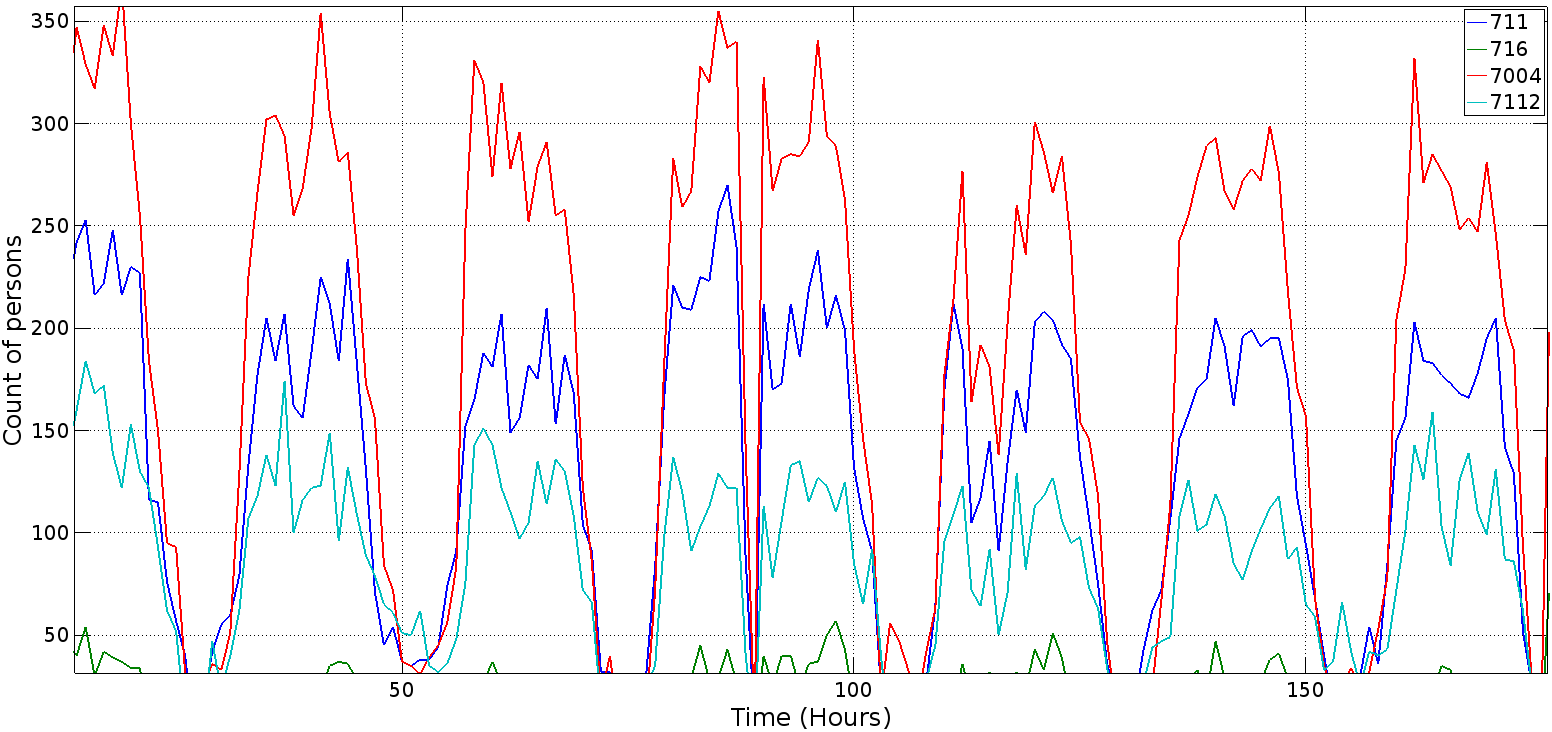
\includegraphics[height=.5\columnwidth]{Figures/Figure_PersonCount_Hours.png}
 \caption{Passenger density evolution over the course of several days.}
  \label{figureHours}
  \end{center}
\end{figure}

We observe that passenger density peaks for the respective cameras are correlated but of different magnitude. 
The overall mean passenger density and standard deviation observed over the same recording time per minute are depicted in Table~\ref{tablePassengerDensity}.

\begin{table}
\begin{center}
\caption{Mean and standard deviation of passenger density data observed at CCTV cameras.}
\label{tablePassengerDensity}
\begin{tabular}{r|ll}
CCTV ID & mean & standard deviation\\\hline
 700 & 1.4816 & 1.5189\\
 701 & 2.1761& 1.8969 \\
704 & 2.8168 & 2.1960\\
705 & 1.8074& 1.8482\\
710 & 2.8167& 3.0868\\
711 & 2.306& 2.1693\\
712 & 2.9604& 2.4585\\
714 & 0.5541& 1.0938 \\
716 & 0.3369& 0.8016\\
720 & 2.6819& 3.046 \\
721 & 1.8885& 2.2247\\
722 & 1.2977& 1.7984\\
731 & 1.7365& 1.8192 \\
732 & 1.3021& 1.5656\\
733 & 1.024& 1.3219\\
7100 & 0.1803& 1.756 \\
7104 & 0.9570& 2.0948\\
7110 & 3.4162& 10.2810\\
7111 & 0.8012& 1.9145\\
7112 & 0.9918& 1.0988\\\hline
\end{tabular}
\end{center}
\end{table}
\pagebreak

\subsection{Prediction by Adaptive Network-based Fuzzy Inference System}
Given the passenger density data provided from the CCTV camera system, we have attempted to predict passenger density with an Adaptive Network-based Fuzzy Inference System (ANFIS)~\cite{Prediction_Jang_1993}.
The ANFIS algorithm was configured to conduct 10 training epochs with a training error goal of 0, an initial step size of 0.01 and step size decrease and increase rates of 0.09 and 1.1 respectively. 

For the training of the system, we utilized data from three consecutive weekdays and attempted to predict the following two days. 
Exemplary prediction results are depicted in Figure~\ref{FigurePrediction} for four distinct CCTV cameras.
The figures show the actual and the predicted evolution of passenger density data.

\begin{figure}
\hspace*{-0.6\columnwidth}% displace figure
\parbox{1.6\columnwidth}{
  \centering
  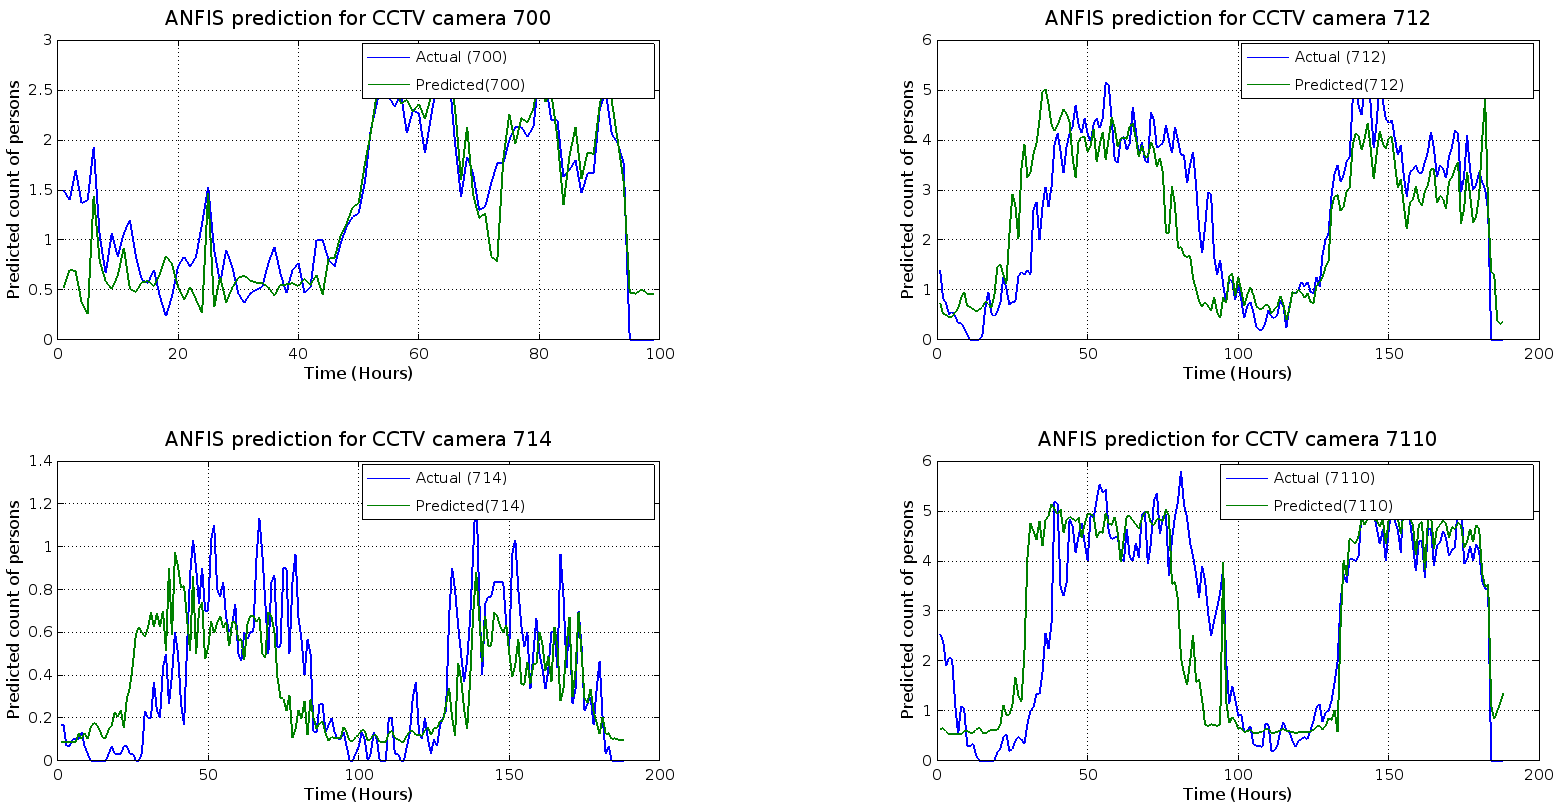
\includegraphics[width=1.6\columnwidth]{Figures/Figure_Prediction.png}
  \caption{ANFIS prediction of passenger density.}
  \label{FigurePrediction}
 }
\end{figure}

We observe that a reasonable prediction accuracy was achieved while the evolution of the predicted sequence often briefly preceded the actual evolution of passenger density.

The prediction error over time is depicted in Figure~\ref{figurePredictionError}.
We observe that the prediction error is low in all cases and near zero.





